\documentclass[a4paper]{article}
\usepackage[T1]{fontenc}			% \chapter package
\usepackage[english]{babel}
\usepackage[english]{isodate}  		% date format
\usepackage{graphicx}				% manage images
\usepackage{amsfonts}
\usepackage{booktabs}				% high quality tables
\usepackage{amsmath}				% math package
\usepackage{amssymb}				% another math package (e.g. \nexists)
\usepackage{bm}                     % bold math symbols
\usepackage{mathtools}				% emphasize equations
\usepackage{stmaryrd} 				% '\llbracket' and '\rrbracket'
\usepackage{amsthm}					% better theorems
\usepackage{enumitem}				% manage list
\usepackage{pifont}					% nice itemize
\usepackage{cancel}					% cancel math equations
\usepackage{caption}				% custom caption
\usepackage[]{mdframed}				% box text
\usepackage{multirow}				% more lines in a table
\usepackage{textcomp, gensymb}		% degree symbol
\usepackage[x11names]{xcolor}		% RGB color
\usepackage{tcolorbox}				% colorful box
\usepackage{multicol}				% more rows in a table (used for the lists)
\usepackage{url}
\usepackage{qrcode}
\usepackage{ragged2e}
\usepackage{cite}                   % references
\usepackage{imakeidx}               % index
\makeindex[program=makeindex, columns=2, 
           title=Index, 
           intoc,
           options={-s index-style.ist}]


% draw a frame around given text
\newcommand{\framedtext}[1]{%
	\par%
	\noindent\fbox{%
		\parbox{\dimexpr\linewidth-2\fboxsep-2\fboxrule}{#1}%
	}%
}


% table of content links
\usepackage{xcolor}
\usepackage[linkcolor=black, citecolor=blue, urlcolor=cyan]{hyperref} % hypertexnames=false
\hypersetup{
	colorlinks=true
}


\newtheorem{theorem}{\textcolor{Red3}{\underline{Theorem}}}
\renewcommand{\qedsymbol}{QED}
\newcommand{\dquotes}[1]{``#1''}
\newcommand{\longline}{\noindent\rule{\textwidth}{0.4pt}}
\newcommand{\circledtext}[1]{\raisebox{.5pt}{\textcircled{\raisebox{-.9pt}{#1}}}}
\newcommand{\definition}[1]{\textcolor{Red3}{\textbf{#1}}\index{#1}}
\newcommand{\example}[1]{\textcolor{Green4}{\textbf{#1}}}
\newcommand{\Var}{\mathrm{Var}}


\begin{document}
    \newcounter{definition}[section]
    \newcounter{example}[section]
    
    \newtcolorbox[use counter = definition]{definitionbox}{%
        colback=red!5!white,
        colframe=red!75!black,
        fonttitle=\bfseries,
        title=Definition \thetcbcounter %
    }
    
    \newtcolorbox[use counter = example]{examplebox}{%
        colback=Green4!5!white,
        colframe=Green4!75!black,
        fonttitle=\bfseries,
        title=Example \thetcbcounter %
    }

    \author{260236}
	\title{Applied Statistics - Notes}
	\date{\printdayoff\today}
	\maketitle

	\newpage

    \section*{Preface}

    Every theory section in these notes has been taken from two sources:
    \begin{itemize}
        \item \href{https://www.statlearning.com/}{An Introduction to Statistical Learning}\cite{james2013introduction}
        \item Applied Multivariate Statistical Analysis (sixth edition).\cite{johnson2007applied}
    \end{itemize}
    
    \newpage
	
	\tableofcontents
	
	\newpage

    \section{Sample Geometry}

    \subsection{The Geometry of the Sample}

    \underline{A single} \definition{multivariate observation} is the \textbf{collection of measurements on $p$ different variables taken on the same item or trial}. If \textbf{$n$ observations} have been obtained, the entire data set can be placed in an $n \times p$ array (or matrix), also called \definition{data frame}:
    \begin{equation}\label{eq: data frame matrix}
        \underset{\left(n \times p\right)}{\mathbf{X}} = \begin{bmatrix}
            x_{11} & x_{12} & \cdots & x_{1p} \\
            x_{21} & x_{22} & \cdots & x_{2p} \\
            \vdots & \vdots & \ddots & \vdots \\
            x_{n1} & x_{n2} & \cdots & x_{np}
        \end{bmatrix}
    \end{equation}
    Each \textbf{row} of $\mathbf{X}$ represents a \textbf{multivariate observation}. Since the entire data frame is often one particular realization of what might have been observed, we say that the data frame are a \textbf{sample of size $n$ from a $p$-variate \dquotes{population}}. The sample then consists of $n$ measurements, each of which has $p$ components.

    Look at the matrix, $n$ measurements (rows), each of which has $p$ components (columns). In mathematics, each $n$ row contains $p$ columns and vice versa.\newline

    \noindent
    The data frame can be plotted in two different ways:
    \begin{enumerate}
        \item $p$-dimensional scatter plot, where the rows represent $n$ points in $p$-dimensional space;
        \item Geometrical representation, $p$ vectors in $n$-dimensional space.
    \end{enumerate}
    
    \longline

    \subsubsection{Scatter plot}

    For the \definition{$p$-dimensional scatter plot}, the rows of $\mathbf{X}$ represent $n$ points in $p$-dimensional space:
    \begin{equation}\label{eq: p-dimensional scatter plot}
        \underset{\left(n \times p\right)}{\mathbf{X}} = \begin{bmatrix}
            x_{11} & x_{12} & \cdots & x_{1p} \\
            x_{21} & x_{22} & \cdots & x_{2p} \\
            \vdots & \vdots & \ddots & \vdots \\
            x_{n1} & x_{n2} & \cdots & x_{np}
        \end{bmatrix} = \left[\begin{array}{@{} c @{}}
            \mathbf{x}_{1}' \\
            \mathbf{x}_{2}' \\
            \vdots \\
            \mathbf{x}_{n}'
        \end{array}\right]
        \begin{array}{l}
            \leftarrow \text{1st (multivariate) observation} \\
            \phantom{\mathbf{x}_{2}'} \\
            \phantom{\vdots} \\
            \leftarrow n\text{th (multivariate) observation}
        \end{array}
    \end{equation}
    The row vector $\mathbf{x}_{j}'$, representing the $j$th observation, contains the coordinates of a point. The \textbf{scatter plot} of $n$ points in $p$-dimensional space \textbf{provides information} on the \textbf{locations and variability of the points}.\newline

    \noindent
    \underline{\textbf{Note}}: when $p$ (dimensional space) is greater than $3$, the \textbf{scatter plot} representation cannot actually be graphed. Yet the consideration of the data as $n$ points in $p$ dimensions provides \textbf{insights that are not readily available from algebraic expressions}.

    \newpage

    \subsubsection{Geometrical representation}

    The alternative \definition{geometrical representation} is constructed by considering the data as \textbf{$p$ vectors in $n$-dimensional space}. Here we take the elements of the columns of the data frame to be the coordinates of the vectors:
    \begin{equation}\label{eq: geometrical representation}
        \underset{\left(n \times p\right)}{\mathbf{X}} = \begin{bmatrix}
            x_{11} & x_{12} & \cdots & x_{1p} \\
            x_{21} & x_{22} & \cdots & x_{2p} \\
            \vdots & \vdots & \ddots & \vdots \\
            x_{n1} & x_{n2} & \cdots & x_{np}
        \end{bmatrix} = \left[\mathbf{y}_{1} \: | \: \mathbf{y}_{2} \: | \: \cdots \: | \: \mathbf{y}_{p}\right]
    \end{equation}
    Then the \textbf{coordinates} of the first point $\mathbf{y}_{1} = \left[x_{11}, x_{21}, \dots, x_{n1}\right]$ \textbf{are the $n$ measurements} on the first variable. 
    
    In general, the $i$th point $\mathbf{y}_{i} = \left[x_{11}, x_{21}, \dots, x_{n1}\right]$ is determined by the $n$-tuple of all measurements on the $i$th variable.\newline

    \noindent
    \textbf{Geometrical representations} usually \textbf{facilitate understanding} and lead to further insights. The ability to \textbf{relate algebraic expressions to the geometric concepts} of length, angle and volume is therefore \textbf{very important}.\newline

    \longline

    \subsubsection{Geometrical interpretation of the process of finding a sample mean}

    Before starting the explanation, you need to understand a few things.
    \begin{itemize}
        \item The \definition{length} of a vector $\mathbf{x}'=\left[x_{1}, x_{2}, \dots, x_{n}\right]$ with $n$ components is defined by:
        \begin{equation}\label{eq: length of a vector}
            L_{x} = \sqrt{x_{1}^{2} + x_{2}^{2} + \cdots + x_{n}^{2}}
        \end{equation}
        Multiplication of a vector $\mathbf{x}$ by a scalar $c$ changes the length:
        \begin{equation*}
            \begin{array}{rcl}
                L_{cx} &=& \sqrt{c^{2} \cdot x_{1}^{2} + c^{2} \cdot x_{2}^{2} + \cdots + c^{2} \cdot x_{n}^{2}} \\ [.3em]
                %
                &=& \left| c \right| \sqrt{x_{1}^{2} + x_{2}^{2} + \cdots + x_{n}^{2}} \\ [.3em] 
                %
                &=& \left| c \right| L_{x}
            \end{array}
        \end{equation*}
        So, for example, in $n = 2$ dimensions, the vector:
        \begin{equation*}
            \mathbf{x} = \begin{bmatrix}
                x_{1} \\ x_{2}
            \end{bmatrix}
        \end{equation*}
        The length of $\mathbf{x}$, written $L_{x}$, is defined to be:
        \begin{equation*}
            L_{x} = \sqrt{x_{1}^{2} + x_{2}^{2}}
        \end{equation*}

        \newpage

        \item Another important concept is \definition{angle}. Consider two vectors in a plane and the angle $\theta$ between them:
        \begin{figure}[!htp]
            \centering
            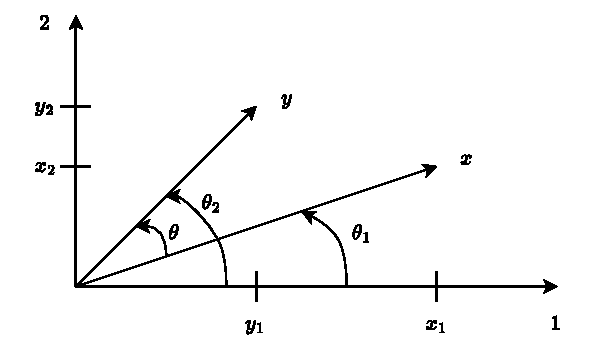
\includegraphics[width=.7\textwidth]{img/basics-vector-algebra-1.pdf}
            \caption{The angle $\theta$ between $\mathbf{x}' = \left[x_{1}, x_{2}\right]$ and $\mathbf{y}' = \left[y_{1}, y_{2}\right]$.}
        \end{figure}
        The value $\theta$ can be represented as the difference between the angles $\theta_{1}$ and $\theta_{2}$ formed by the two vectors and the first coordinate axis. Since, by definition:
        \begin{gather*}
            \begin{array}{rcl}
                \cos\left(\theta_{1}\right) = \dfrac{x_{1}}{L_{x}} & \cos\left(\theta_{2}\right) = \dfrac{y_{1}}{L_{y}} \\ [1em]
                %
                \sin\left(\theta_{1}\right) = \dfrac{x_{2}}{L_{x}} & \sin\left(\theta_{2}\right) = \dfrac{y_{2}}{L_{y}}
            \end{array} \\
            \cos\left(\theta\right) = \cos\left(\theta_{2} - \theta_{1}\right) = \cos\left(\theta_{2}\right) \cos\left(\theta_{1}\right) + \sin\left(\theta_{2}\right) \sin\left(\theta_{1}\right)
        \end{gather*}
        The angle $\theta$ between the two vectors $\mathbf{x}' = \left[x_{1}, x_{2}\right]$ and $\mathbf{y}' = \left[y_{1}, y_{2}\right]$ is specified by:
        \begin{equation}\label{eq: angle}
            \cos\left(\theta\right) = \cos\left(\theta_{2} - \theta_{1}\right) = 
            \left(\dfrac{y_{1}}{L_{y}}\right)\left(\dfrac{x_{1}}{L_{x}}\right) + \left(\dfrac{y_{2}}{L_{y}}\right)\left(\dfrac{x^{2}}{L_{x}}\right) =
            \dfrac{x_{1}y_{1} + x_{2}y_{2}}{L_{x}L_{y}}
        \end{equation}

        \item With the angle equation~\ref{eq: angle}, it's convenient to introduce the \definition{inner product} of two vectors:
        \begin{equation*}
            \mathbf{x}\mathbf{y}' = x_{1}y_{1} + x_{2}y_{2}
        \end{equation*}
        So let us rewrite:
        \begin{itemize}
            \item The \textbf{length} equation~\ref{eq: length of a vector}:
            \begin{equation}\label{eq: length rewritten with inner product}
                \mathbf{x}'\mathbf{x} = x_{1} x_{1} + x_{1} x_{1} = x_{1}^{2} + x_{2}^{2} 
                \longrightarrow
                L_{x} = \sqrt{x_{1}^{2} + x_{2}^{2}}
                \Longrightarrow
                L_{x} = \sqrt{\mathbf{x}' \mathbf{x}}
            \end{equation}

            \item The \textbf{angle} equation~\ref{eq: angle}:
            \begin{equation*}
                \cos\left(\theta\right) = \dfrac{x_{1}y_{1} + x_{2}y_{2}}{L_{x}L_{y}} 
                \Longrightarrow
                \cos\left(\theta\right) = \dfrac{\mathbf{x}'\mathbf{y}}{L_{x}L_{y}}
            \end{equation*}
            And using the rewritten length equation:
            \begin{equation*}
                \cos\left(\theta\right) = \dfrac{\mathbf{x}'\mathbf{y}}{L_{x}L_{y}} \Longrightarrow
                \cos\left(\theta\right) = \dfrac{\mathbf{x}'\mathbf{y}}{\sqrt{\mathbf{x}' \mathbf{x}} \cdot \sqrt{\mathbf{y}' \mathbf{y}}}
            \end{equation*}
        \end{itemize}
        
        \item The \definition{projection} (or shadown) of a vector $\mathbf{x}$ on a vector $\mathbf{y}$ is:
        \begin{equation}\label{eq: projection}
            \dfrac{\left(\mathbf{x}'\mathbf{y}\right)}{\mathbf{y}'\mathbf{y}}\mathbf{y} = \dfrac{\left(\mathbf{x}'\mathbf{y}\right)}{L_{y}}\dfrac{1}{L_{y}}\mathbf{y}
        \end{equation}
        Where the vector $\dfrac{1}{L_{y}}\mathbf{y}$ has unit length. The \textbf{length of the projection} is:
        \begin{equation}\label{eq: length of the projection}
            \dfrac{\left| \mathbf{x}'\mathbf{y} \right|}{L_{y}} = L_{x} \left| \dfrac{\mathbf{x}'\mathbf{y}}{L_{x}L_{y}} \right| = L_{x} \left| \cos\left(\theta\right) \right|
        \end{equation}
        Where $\theta$ is the angle between $\mathbf{x}$ and $\mathbf{y}$:
        \begin{figure}[!htp]
            \centering
            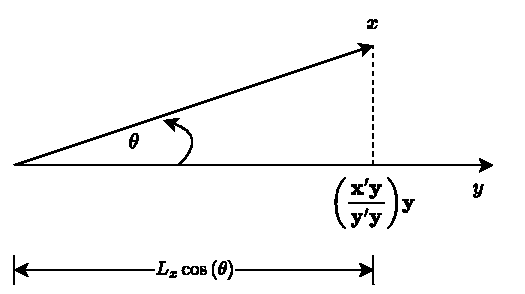
\includegraphics[width=.7\textwidth]{img/basics-vector-algebra-2.pdf}
            \caption{The projection of $\mathbf{x}$ on $\mathbf{y}$.}
        \end{figure}
    \end{itemize}
    Start by defining the $n \times 1$ vector $\mathbf{1}_{n}' = \left[1, 1, \dots, 1\right]$. The vector $\mathbf{1}$ forms equal angles with each of the $n$ coordinates axes, so the vector $\left(\dfrac{1}{\sqrt{n}}\right)\mathbf{1}$ has unit length in the equal-angle direction. Consider the vector $\mathbf{y}_{i}' = \left[x_{1i}, x_{2i}, \dots, x_{ni}\right]$. The projection of $\mathbf{y}_{i}$ on the unit vector $\left(\dfrac{1}{\sqrt{n}}\right)\mathbf{1}$ is:
    \begin{equation}\label{eq: sample mean - geometrical representation}
        \mathbf{y}_{i}'\left(\dfrac{1}{\sqrt{n}}\mathbf{1}\right)\dfrac{1}{\sqrt{n}}\mathbf{1} = 
        \dfrac{x_{1i} + x_{2i} + \cdots + x_{ni}}{n}\mathbf{1} = \overline{x}_{i}\mathbf{1}
    \end{equation}
    Although it may seem like a complex equation at first glance, it is nothing more than the mean! In fact, the \textbf{sample mean} $\overline{\mathbf{x}}_{i} = \dfrac{\left(x_{1i} + x_{2i} + \cdots + x_{ni}\right)}{n} = \dfrac{\mathbf{y}_{i}' \mathbf{1}}{n}$ corresponds to the multiple of $\mathbf{1}$ required to give the projection of $\mathbf{y}_{i}$ onto the line determined by $\mathbf{1}$.\newpage

    \noindent
    Furthermore, using the projection, you can obtain the \textbf{deviation} (\textbf{mean corrected}). For each $\mathbf{y}_{i}$ we have the decomposition:
    \begin{figure}[!htp]
        \centering
        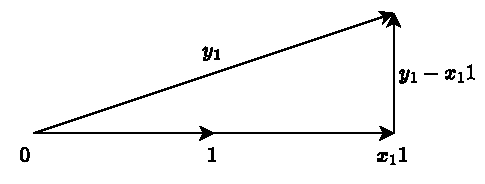
\includegraphics[width=.6\textwidth]{img/basics-vector-algebra-3.pdf}
    \end{figure}

    \noindent
    Where $\overline{x}_{i} \mathbf{1}$ is perpendicular to $y_{i}-\overline{x}_{i}\mathbf{1}$. The \definition{deviation}, or \definition{mean corrected}, vector is:
    \begin{equation}\label{eq: deviation - mean corrected}
        \mathbf{d}_{i} = \mathbf{y}_{i} - \overline{x}_{i}\mathbf{1} = \begin{bmatrix}
            x_{1i} - \overline{x}_{i} \\
            x_{2i} - \overline{x}_{i} \\
            \vdots \\
            x_{ni} - \overline{x}_{i}
        \end{bmatrix}
    \end{equation}
    The \textbf{elements} of $\mathbf{d}_{i}$ are the \textbf{deviations of the measurements on the $i$th variable from their sample mean}.\newline

    \noindent
    Using the length rewritten with inner product (equation~\ref{eq: length rewritten with inner product}) and the deviation (equation~\ref{eq: deviation - mean corrected}), we obtain:
    \begin{equation}
        L_{\mathbf{d}_{i}}^{2} = \mathbf{d}_{i}'\mathbf{d}_{i} = \displaystyle\sum_{j=1}^{n}\left(x_{ji}-\overline{x}_{i}\right)^{2}
    \end{equation}
    \begin{equation*}
        \left(\text{Length of deviation vector}\right)^{2} = \text{sum of squared deviations}
    \end{equation*}
    From the sample standard deviation, we see that the \textbf{squared length is proportional to the variance} of the measurements on the $i$th variable. Equivalently, the \textbf{length is proportional to the standard deviation}. So longer vectors represent more variability than shorter vectors.

    Furthermore, for any two deviation vectors $\mathbf{d}_{i}$ and $\mathbf{d}_{k}$:
    \begin{equation}
        \mathbf{d}_{i}'\mathbf{d}_{k} = \displaystyle\sum_{j=1}^{n}\left(x_{ji} - \overline{x}_{i}\right)\left(x_{jk} - \overline{x}_{k}\right)
    \end{equation}
    And with a few mathematical operations, we can get it:
    \begin{equation}
        r_{ik} = \dfrac{s_{ik}}{\sqrt{s_{ii}}\sqrt{s_{kk}}} = \cos\left(\theta_{ik}\right)
    \end{equation}
    Where the \textbf{cosine} of the angle is the \definition{sample correlation coefficient}. Note: $s_{ik}$ is the \definition{sample covariance}:
    \begin{equation}\label{eq: sample covariance}
        s_{ik} = \dfrac{1}{n} \displaystyle\sum_{j=1}^{n} \left(x_{ji} - \overline{x}_{i}\right)\left(x_{jk} - \overline{x}_{k}\right) \hspace{2em} i = 1,2,\dots,p, \hspace{1em} k = 1,2,\dots,p
    \end{equation}
    Thus:
    \begin{itemize}
        \item If the two deviation vectors have \textbf{nearly the same orientation}, the sample correlation will be close to $1$;
        \item If the two vectors are \textbf{nearly perpendicular}, the sample correlation will be approximately zero;
        \item If the two vectors are oriented in \textbf{nearly opposite directions}, the sample correlation will be close to $-1$.
    \end{itemize}

    \longline

    \subsection{Generalized Variance}

    Before starting the explanation, you need to understand what is a sample variance.

    A \definition{sample variance} is defined as:
    \begin{equation}\label{eq: sample variance}
        s_{k}^{2} = s_{kk} = \dfrac{1}{n-1} \displaystyle\sum_{j=1}^{n} \left(x_{jk} - \overline{x}_{k}\right)^{2} \hspace{2em} k = 1, 2, \dots, p
    \end{equation}

    With a single variable, the \textbf{sample variance is often used to describe the amount of variation in the measurements on that variable}. When $p$ variables are observed on each unit, the variation is described by the \definition{sample variance-covariance matrix}:
    \begin{equation}
        \mathbf{S} = \begin{bmatrix}
            s_{11} & s_{12} & \cdots & s_{1p} \\
            s_{21} & s_{22} & \cdots & s_{2p} \\
            \vdots & \vdots & \ddots & \vdots \\
            s_{p1} & s_{p2} & \cdots & s_{pp}
        \end{bmatrix} =
        \left\{s_{ik} = \dfrac{1}{n-1}\displaystyle\sum_{j=1}^{n}\left(x_{ji}-\overline{x}_{i}\right)\left(x_{jk}-\overline{x}_{k}\right)\right\}
    \end{equation}
    The sample covariance matrix contains $p$ variances and $\dfrac{1}{2}p\left(p-1\right)$ potentially different covariances. Sometimes it's desirable to \textbf{assign a single numerical value for the variation expressed by $\mathbf{S}$}. One choice for a value is the \href{https://en.wikipedia.org/wiki/Determinant}{determinant} of $\mathbf{S}$, which reduces to the usual sample variance of a single characteristic when $p=1$. This determinant is called the \definition{generalized sample variance}:
    \begin{equation}
        \text{Generalized sample variance} = \det\left(\mathbf{S}\right) = \left| \mathbf{S} \right|
    \end{equation}
    
    \newpage

    \section{Statistical Learning}

    \subsection{Introduction}

    Suppose that we observe a quantitative response $Y$ and $p$ different predictors, $X_{1}, X_{2}, \dots, X_{p}$. We assume that there is some relationship between $Y$ and $X = \left(X_{1}, X_{2}, \dots, X_{p}\right)$, which can be written in the general form:
    \begin{equation}
        Y = f\left(X\right) + \varepsilon
    \end{equation}
    Where $\varepsilon$ is an \definition{error term}, which is \textbf{independent} of $X$ and has \textbf{mean zero}. The function $f$ represents the \definition{systematic information} that $X$ provides about $Y$. The \textbf{function} $f$ that connects the input variables to the output variable \textbf{is in general unknown}.
    
    \begin{examplebox}
        For \example{example}, on the left-hand panel of figure~\ref{fig: error term systematic}, a plot \texttt{income} versus \texttt{years of education} for 30 individuals in the Income data set.
        
        \begin{center}
            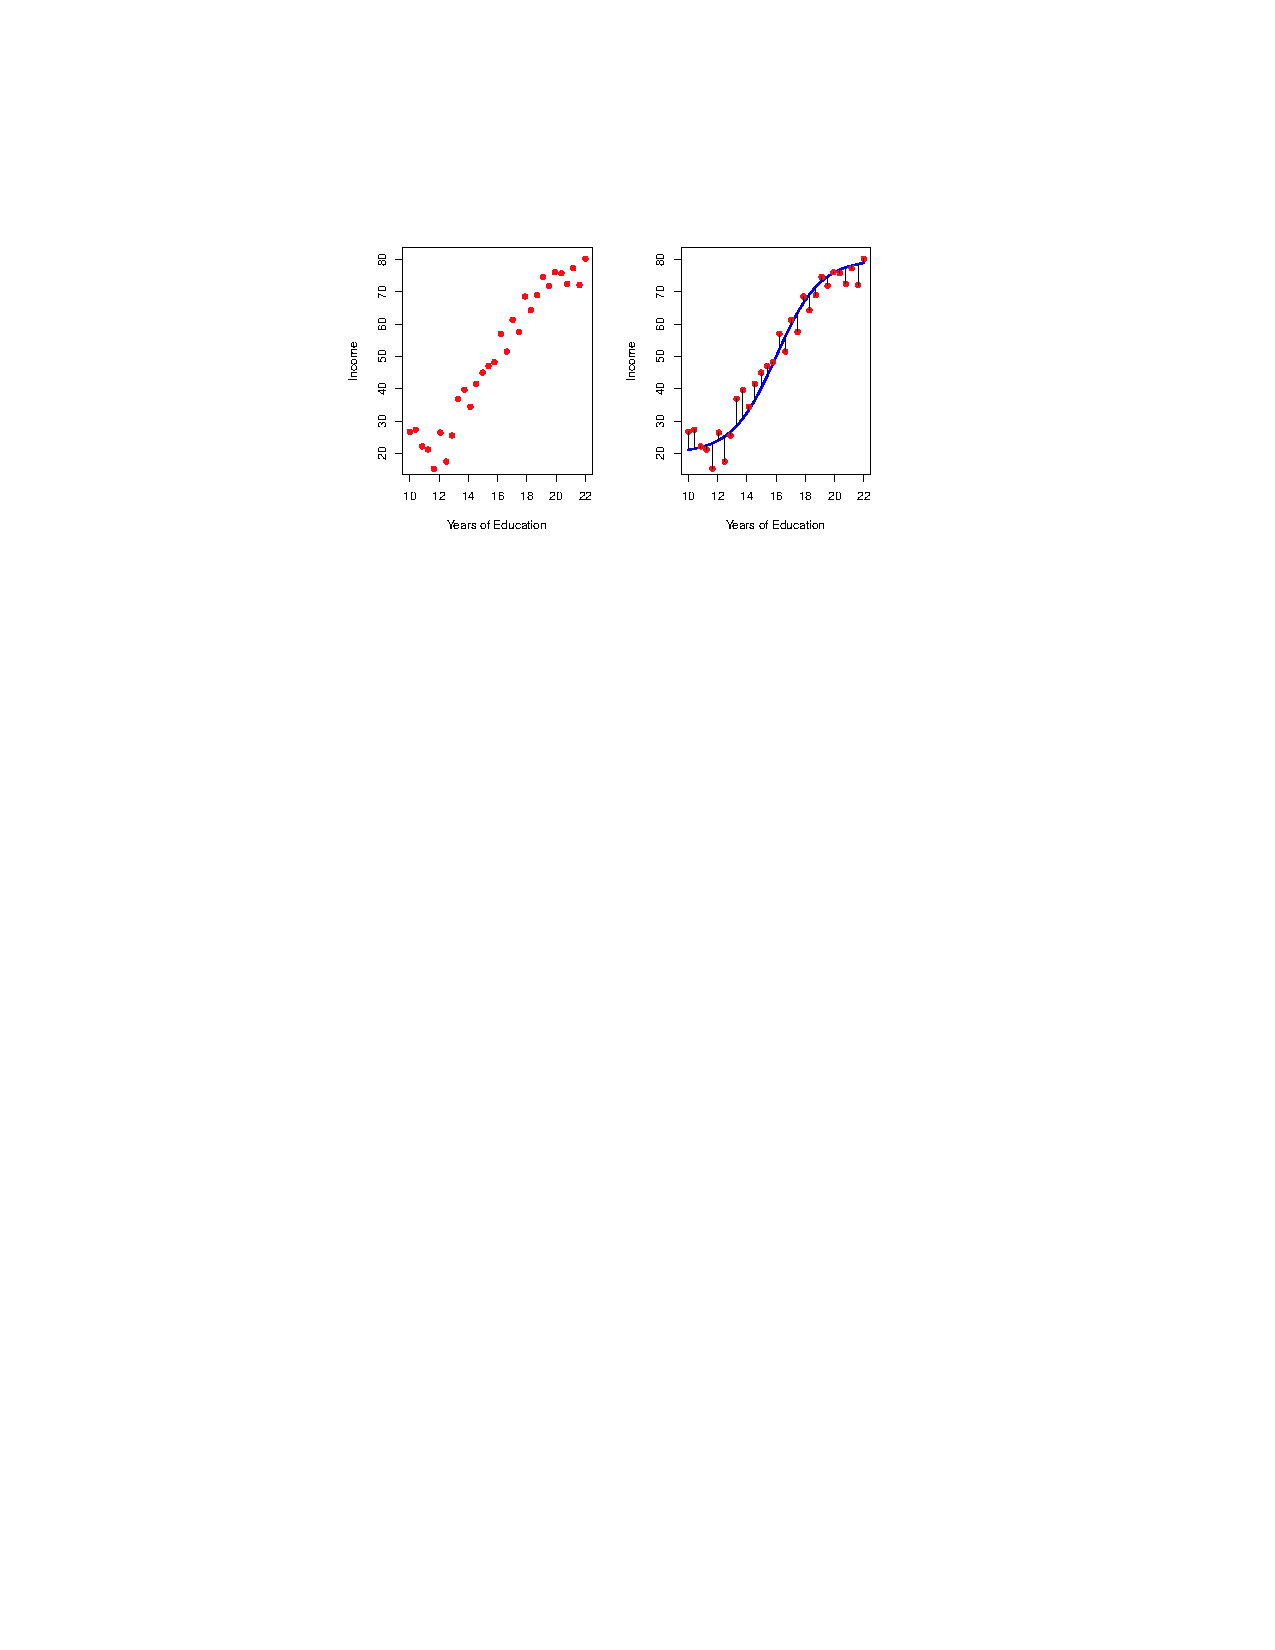
\includegraphics[width=\textwidth]{img/error-term-systematic-1.pdf}
            \captionof{figure}{The \texttt{Income} data set.\cite{james2013introduction}}
            \label{fig: error term systematic}
        \end{center}


        \noindent
        As you can see, the plot suggests that one might be able to predict \texttt{income} using \texttt{years of education}. Since \texttt{Income} is a simulated data set, the function $f$ is known and is shown by the blue curve in the right-hand panel. The \textbf{vertical lines} represent the \textbf{error terms} $\varepsilon$. We note that some of the 30 observations lie above the blue curve and some lie below it; overall, the \textbf{errors have approximately mean zero}.
    \end{examplebox}

    \noindent
    In essence, \textbf{statistical learning refers to a set of approaches for estimating $f$}. In this chapter we outline some of the key theoretical concepts that arise in estimating $f$.

    \newpage

    \subsection{Why Estimate \emph{f} (systematic information provided by a predictor about a quantitative response)?}

    There are two main reasons that we may wish to estimate $f$\index{systematic information}: \definition{prediction} and \definition{inference}.

    \longline

    \subsubsection{Prediction}

    In many situations, a set of inputs $X$ are readily available, but the output $Y$ cannot be easily obtained. In this setting, since the error term $\varepsilon$ averages to zero, we can predict $Y$ using:
    \begin{equation}
        \hat{Y} = \hat{f}\left(X\right)
    \end{equation}
    \begin{itemize}
        \item $\hat{f}$ represents our \textbf{estimate for} $\bm{f}$
        \item $\hat{Y}$ represents \definition{prediction} for $Y$
    \end{itemize}
    The function $\hat{f}$ is often treated as a \textbf{black box}, in the sense that one is not typically concerned with the exact form of $\hat{f}$, provided that \textbf{it yields accurate predictions for} $Y$.

    \begin{examplebox}
        As an \example{example}, suppose that:
        \begin{itemize}
            \item $X_{1}, \dots, X_{p}$ are \textbf{characteristics of a patient's blood sample} that can be easily measured in a lab.
            \item $Y$ is a variable encoding the \textbf{patient's risk for a severe adverse reaction to a particular drug}.
        \end{itemize}
        It is natural to seek to predict $Y$ using $X$, since we can then avoid giving the drug in question to patients who are at high risk of an adverse reaction. That is, patients for whom the estimate of $Y$ is high.
    \end{examplebox}

    \noindent
    The accuracy of $\hat{Y}$ as a prediction for $Y$ depends on two quantities: \definition{reducible error} and \definition{irreducible error}.
    \begin{itemize}
        \item In general, $\hat{f}$ will not be a perfect estimate for $f$, and this \textbf{inaccuracy} will introduce some error. This is a \definition{reducible error} because we can potentially \textbf{improve the accuracy of $\bm{\hat{f}}$ by using the most appropriate statistical learning technique to estimate $\bm{f}$}.
        
        \item Even if it were possible to form a perfect estimate for $f$, so that our estimated response took the form $\hat{Y} = f\left(X\right)$, our prediction would still have some error in it! This is because $Y$ is also a function of $\varepsilon$ (error term), which, by definition, cannot be predicted using $X$. Therefore, variability associated with $\varepsilon$ also affects the accuracy of our predictions. This is the \definition{irreducible error}, because \textbf{no matter how well we estimate $\bm{f}$, we cannot reduce the error introduced by $\bm{\varepsilon}$}.
    \end{itemize}
    The real question is: \emph{why is the irreducible error larger than zero?} Well, the quantity $\varepsilon$ may contain unmeasured variables that are useful in predicting $Y$: since we don't measure them, $f$ cannot use them for its prediction. The quantity $\varepsilon$ may also contain unmeasurable variation.

    \begin{examplebox}
        For \example{example}, the risk of an adverse reaction might vary for a given patient on a given day, depending on manufacturing variation in the drug itself or the patient's general feeling of well-being on that day.
    \end{examplebox}

    \noindent
    Consider a given estimate $\hat{f}$ and a set of predictors $X$, which yields the prediction $\hat{Y} = \hat{f}\left(X\right)$. Assume for a moment that both $\hat{f}$ and $X$ are fixed, so that the only variability comes from $\varepsilon$ (error term). Then, it's easy to show that:
    \begin{equation}
        \begin{array}{rcl}
            E\left(Y - \hat{Y}\right)^{2} &=& E\left[f\left(X\right) + \varepsilon - \hat{f}\left(X\right)\right]^{2} \\ [1em]
                                          &=& \underbrace{\left[f\left(X\right) - \hat{f}\left(X\right)\right]^{2}}_{\text{Reducible}} + \underbrace{\Var\left(\varepsilon\right)}_{\text{Irreducible}}
        \end{array}
    \end{equation}
    \begin{itemize}
        \item $\left[f\left(X\right) - \hat{f}\left(X\right)\right]^{2}$ represents the \textbf{squared difference between the predicted and actual value of} $\bm{Y}$
        
        \item $E\left(Y-\hat{Y}\right)^{2}$ represents the \textbf{average}, or \definition{exprected value}
        
        \item $\Var\left(\varepsilon\right)$ represents the \definition{variance} \textbf{associated with the error term} $\varepsilon$
    \end{itemize}













    %%%%%%%%%%%%%%%%%%%%%%%%%%%%%%%%%%%%%%%%%%%%%%%%%%%%%%%%%%%%%%%%%%%%%%%%%%%%%%%%%%%%%%%%%
    %%%%%%%%%%%%%%%%%%%%%%%%%%%%%%%%%%%%%%%%%%%%%%%%%%%%%%%%%%%%%%%%%%%%%%%%%%%%%%%%%%%%%%%%%
    %%%%%%%%%%%%%%%%%%%%%%%%%%%%%%%%%%%%%%%%%% END %%%%%%%%%%%%%%%%%%%%%%%%%%%%%%%%%%%%%%%%%%
    %%%%%%%%%%%%%%%%%%%%%%%%%%%%%%%%%%%%%%%%%%%%%%%%%%%%%%%%%%%%%%%%%%%%%%%%%%%%%%%%%%%%%%%%%
    %%%%%%%%%%%%%%%%%%%%%%%%%%%%%%%%%%%%%%%%%%%%%%%%%%%%%%%%%%%%%%%%%%%%%%%%%%%%%%%%%%%%%%%%%


    \newpage

    \bibliography{bibtex}{}
    \bibliographystyle{plain}

    \newpage

    \printindex
\end{document}